\documentclass[00_doc.tex]{subfiles}
\begin{document}
    \subsection{Merging Code and Physical Components}
    \begin{flushleft}
        After coding everything and testing the code if everything is working as we wanted, we glued
        the blossom and the base together and connected the copper foil to the base. Therefore, we had 
        to drill some holes in the ground, so wires can be added. The final prototype of the be seen in 
        Figure ~\ref{fig:finalPrototyp}.
    \end{flushleft}

    \begin{table}[h!]
        \centering
        \begin{tabular}{c}
        \centering
        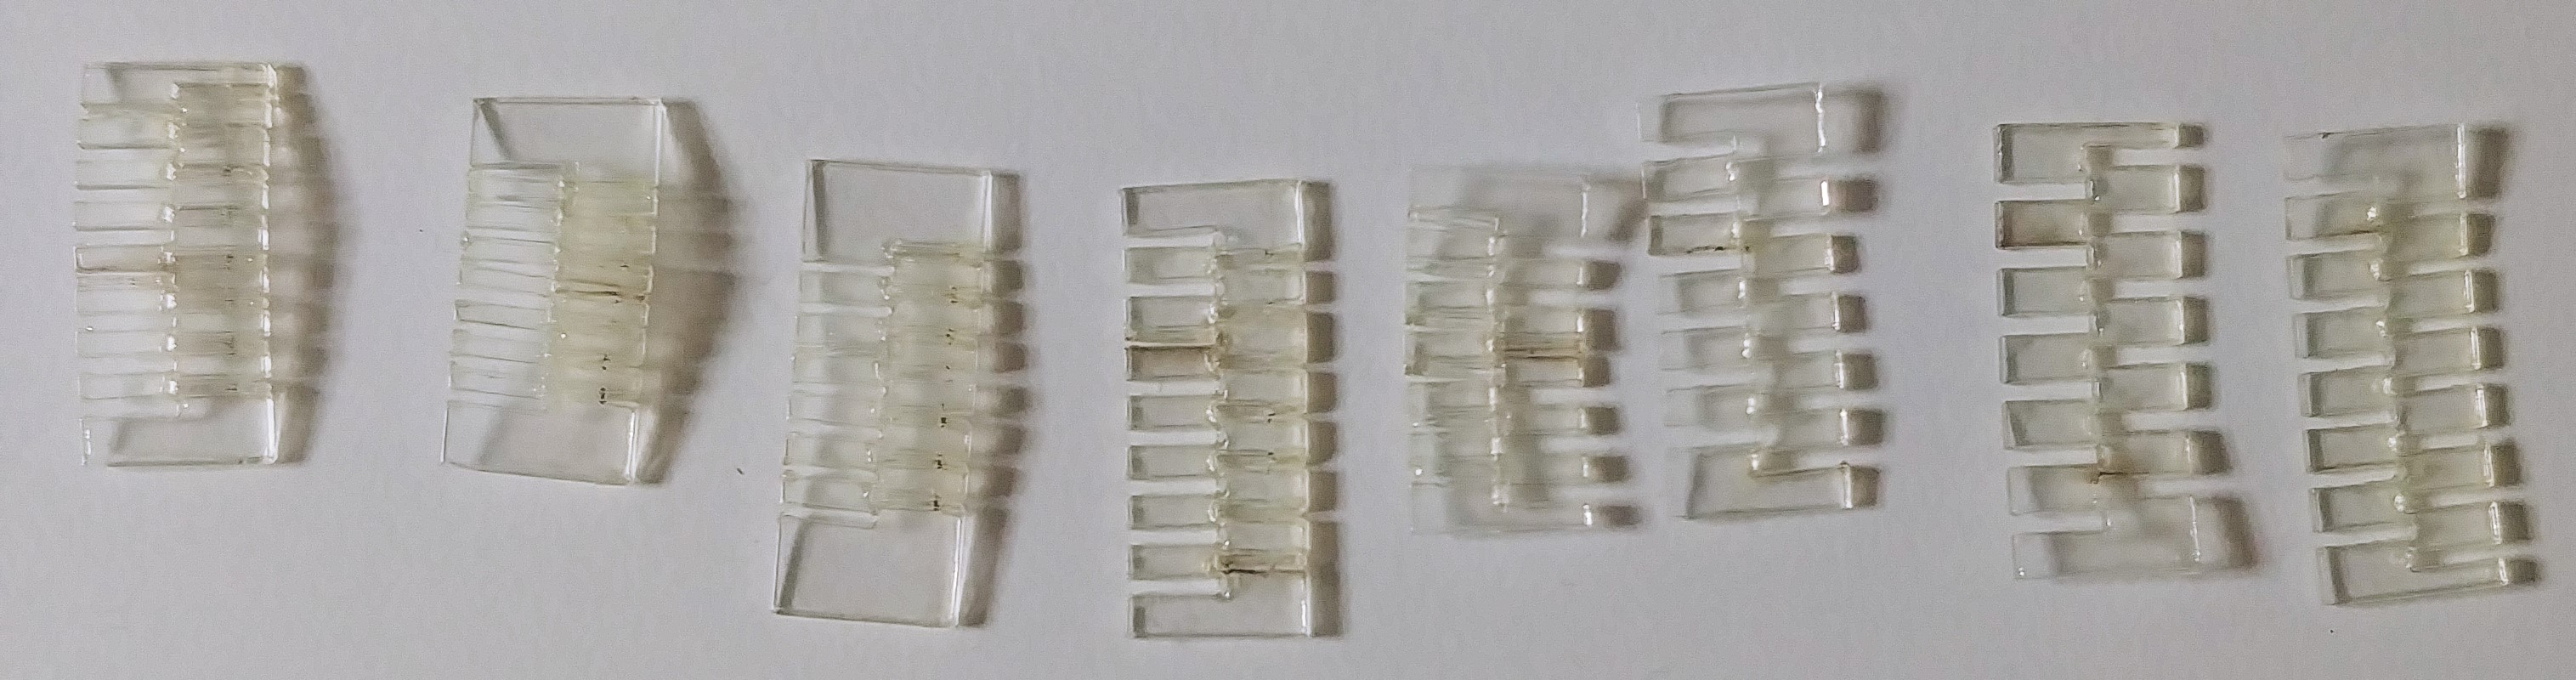
\includegraphics[width=.8\linewidth]{images/process/01_LaserCut.jpg}
        \end{tabular}
        \caption{Shows the final prototyp of the blossom shaped lamp}
        \label{fig:finalPrototyp}
    \end{table}
\end{document}
